\documentclass[12pt]{article}
\usepackage[margin=1in]{geometry}
\usepackage{enumitem}
\usepackage{titlesec}
\usepackage{parskip}
\usepackage{graphicx}
\usepackage{hyperref}
\usepackage{fontenc}

\title{\textbf{Carey 2009 RG Notes}\\
\large Carey, John M. \textit{Legislative Voting and Accountability}.\\
Cambridge: Cambridge University Press, 2009.}
\author{}
\date{}

\begin{document}

\maketitle

\section{Main Idea}



%--------------------------------------------------
\section{General Notes}
%--------------------------------------------------

\begin{itemize}[leftmargin=*, itemsep=4pt]
    \item Differentiation between collective and individualistic accountability: an entire legislature or governing party can relatively easily be held accountable by voters for policy \emph{outcomes}, as they are supposedly entrusted with delivering productive results. Yet, it can be difficult for voters to obtain information on specific legislators such that they may be held accountable for their more specific actions. This is a fundamental informational tradeoff delineating two frameworks of legislative accountability.'
    \item Legislators face two primary \textbf{and competing} principals (likely more): their voters can hold them accountable, especially if individualistic accountability is possible, and their party leadership can hold them accountable depending on the institutional strength of the party system. (A high-ranking third principal would be presidents because of their impact on legislative outcomes and processes). These principals may be sequential (i.e., voters $\rightarrow$ parties $\rightarrow$ legislator) or competing (i.e., voters $\rightarrow$ parties $\rightarrow$ legislator AND voters $\rightarrow$ legislator)
    \begin{center}
        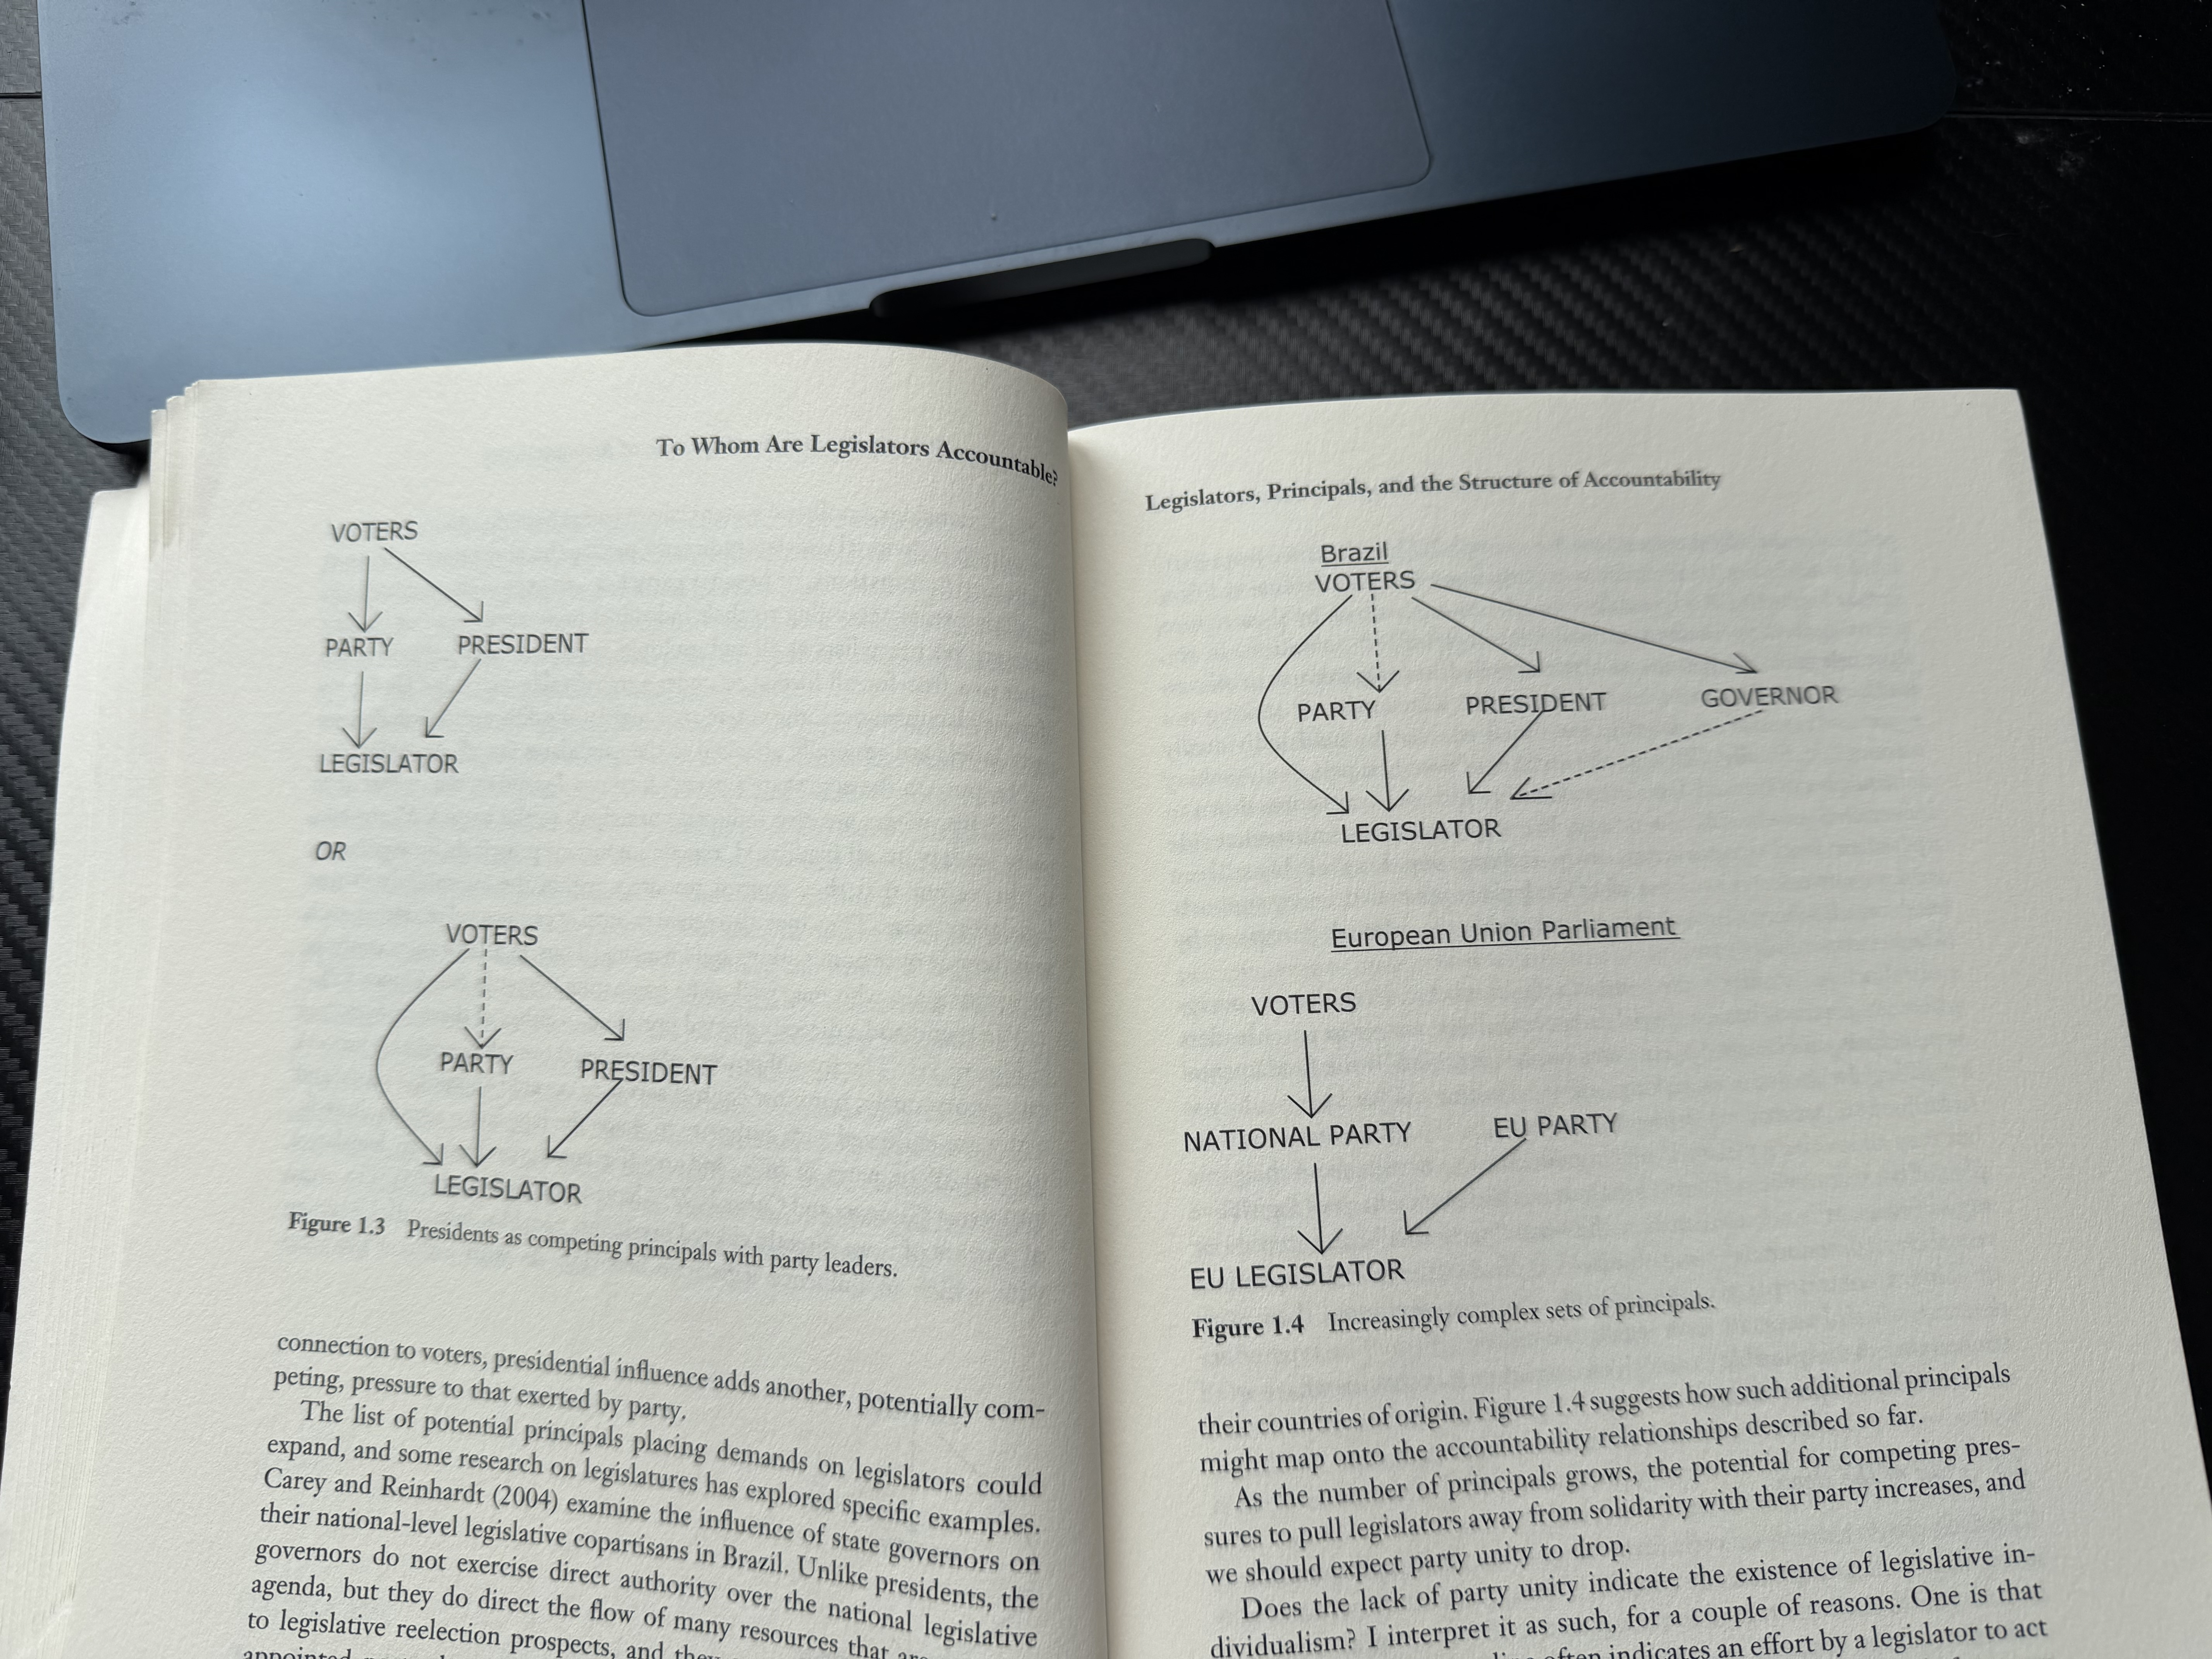
\includegraphics[width=13cm]{principal models.jpg}
    \end{center}
    \item Parties become less unified as the number and magnitude of principals increases; unity as an equilibrium outcome instead of a fixed trait
    \item Parties incur costs by disciplining their members -- both from the administration of said costs, but also because it limits individual members' abilities to garner local support which could then more broadly be translated into party support. (This is potentially a Fetterman-esque situation -- if you believe it is more likely that he will vote with the Democrats on some key issues, it may be worthwhile for him to stray further so long as it secures a Democratic seat in Pennsylvania)
    \item Driving question: are votes visible? If individual votes can be tracked and accurately reported, then the likelihood of voters being able to pursue individualistic accountability is much greater (though still contingent on the institutional means of actually doing so -- that is, how they are able to inflict electoral consequence). But, if individual votes cannot be tracked or reported -- for example, via anonymity, voice votes, etc. -- it can become exceedingly difficult for this mechanism to be maintained.
    \begin{itemize}
        \item It is also important to distinguish between \emph{who} can observe these individual votes. In cases where that information may not be made available to voters, it still could be possible for party leaders to identify behaviors internally.
        \item Notes that transparency is not unilaterally a productive thing, as it can weaken collective accountability and (extension) can create adverse incentives against good governance. \textbf{Transparency redistributes accountability instead of plainly increasing it}
    \end{itemize}
    \item Empirical analysis: party unity on roll-call votes, primarily using the RICE index (absolute difference between the shares of a party voting Y/N on a given vote)
\end{itemize}


\section{Important Specific Factual Claims}

\begin{itemize}[leftmargin=*, itemsep=4pt]
    \item Legislators face decisiveness problems:
    \begin{itemize}
        \item \underline{Bottlenecks}: There are an infinite (or at least, very large) number of policy options available for any given question, and legislatures must narrow down to some much smaller range of viable alternatives from which to collectively choose. Parties may be a solution to this, in identifying specific policy alternatives as being the general linkage to their own ideological background. However, this also implies limiting the agenda-setting capacity of many legislative actors such that an unbreakable stalemate can be avoided; similarly, veto players must be limited in order to prevent cycling or instability.
        \item \underline{Promotion}: As a legislator becomes more experienced and gains seniority, they both gain access to additional decision-making power and decrease their vulnerability to replacement (this is especially true in party-list elections). This accountability mechanism may subsequently become weaker, requiring alternative forms of punishment/consequence.
        \item ``Party unity is the point of reference because legislators everywhere are partisan, because legislators everywhere answer to party leaders as principals, and because party unity can be identified by the fundamental act of legislative decision making -- that is, voting. Where party unity is lacking, there are various stories we can tell about legislative motivation, but they all involve legislators' making decisions to deviate from the game plan of the team -- the collective unit -- that is the central basis of legislative organization.'
    \end{itemize}
\end{itemize}


\section{Connections}

\begin{itemize}
    \item Accountability requires both responsiveness, information about behavior, and the ability to act on that information -- very aligned w/ Powell? (check which author this was)
    \item Critiques typical construction of an SMDP vs. PR tradeoff (explicitly naming Lijphart and Huber/Powell): ``This conclusion rests on two key assumptions, however: that political parties are fundamental units of legislative representation and that a left-right spectrum meaningfully describes the ideological arena of party competition. They are open to greater skepticism in environments where party systems are more volatile or party reputations less stable.'' Claims that the fundamental tradeoff instead should be between whether or not accountability is collective or individualistic (which is itself a downstream impact of the majoritarianism vs. proportionalism debate).
    \item When considering the impact of observability on accountability -- ties very closely to Stokes et al, who suggest that perceiving individual votes (outside of the legislature and instead at the citizenry level) may actually be significantly easier than previously thought, or at least, that voters believe it to be quite possible.
    \item Larreguy \& Raffler 2025 discuss two nested principal-agent problems within developing democracies -- voters and politicians, and politicians and bureaucrats. Contrast however that this is directional rather than doubled-up -- but, the rest of the paper has many citations to be considered here as well
\end{itemize}


\section{My Critiques}

\begin{itemize}
    \item 
\end{itemize}


\end{document}
